\section{Polar Form and Euler's Formula}
\label{sec:ch5-polar-euler}

For $z\neq0$, define $r=|z|$ and an argument $\theta$ by
\[
x=r\cos\theta,\qquad y=r\sin\theta.
\]
Then
\[
z=r(\cos\theta+i\sin\theta).
\]
The argument is multivalued: $\theta$ and $\theta+2\pi n$ describe the same point. A selected representative is called a principal argument.

\begin{figure}[htbp]
\centering
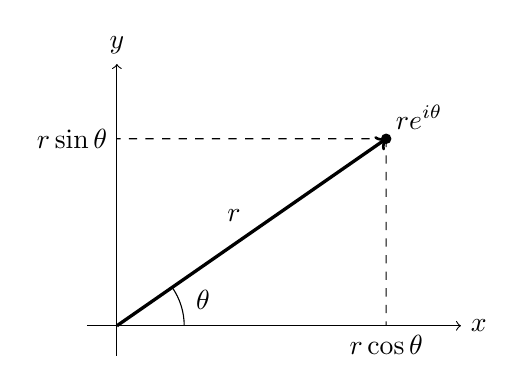
\begin{tikzpicture}[scale=0.95]
\draw[->] (-0.4,0)--(4.6,0) node[right] {$x$};
\draw[->] (0,-0.4)--(0,3.5) node[above] {$y$};
\coordinate (Z) at (3.6,2.5);
\draw[->,very thick] (0,0)--(Z) node[midway,above left] {$r$};
\draw[dashed] (Z)--(3.6,0); \draw[dashed] (Z)--(0,2.5);
\draw (0.9,0) arc (0:34.8:0.9); \node at (1.15,0.35) {$\theta$};
\fill (Z) circle (2pt) node[above right] {$re^{i\theta}$};
\node[below] at (3.6,0) {$r\cos\theta$}; \node[left] at (0,2.5) {$r\sin\theta$};
\end{tikzpicture}

\caption{Cartesian and polar descriptions of the same complex number.}
\label{fig:ch5-polar}
\end{figure}

Euler's formula states
\[
\boxed{e^{i\theta}=\cos\theta+i\sin\theta}.
\]
Comparing power series gives
\begin{align}
e^{i\theta}
&=1+i\theta+\frac{(i\theta)^2}{2!}+\frac{(i\theta)^3}{3!}+\cdots\\
&=\left(1-\frac{\theta^2}{2!}+\frac{\theta^4}{4!}-\cdots\right)
+i\left(\theta-\frac{\theta^3}{3!}+\frac{\theta^5}{5!}-\cdots\right).
\end{align}
Thus
\[
\boxed{z=re^{i\theta}}.
\]

\begin{keyidea}[Oscillation is rotation viewed from one axis]
The point $e^{i\omega t}$ moves uniformly around the unit circle. Its real projection is $\cos\omega t$ and its imaginary projection is $\sin\omega t$. Harmonic motion is a shadow of uniform rotation in the complex plane.
\end{keyidea}

\begin{figure}[htbp]
\centering
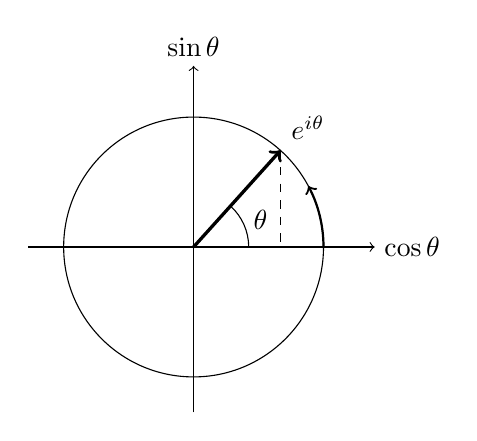
\begin{tikzpicture}[scale=1.0]
\draw[->] (-2.1,0)--(2.3,0) node[right] {$\cos\theta$};
\draw[->] (0,-2.1)--(0,2.3) node[above] {$\sin\theta$};
\draw (0,0) circle (1.65);
\coordinate (P) at ({1.65*cos(48)},{1.65*sin(48)});
\draw[->,very thick] (0,0)--(P) node[above right] {$e^{i\theta}$};
\draw[dashed] (P)--({1.65*cos(48)},0);
\draw (0.7,0) arc (0:48:0.7); \node at (0.85,0.35) {$\theta$};
\draw[->,thick] (1.65,0) arc (0:28:1.65);
\end{tikzpicture}

\caption{Uniform complex rotation generates sine and cosine as coordinate projections.}
\label{fig:ch5-euler-rotation}
\end{figure}

The identity $e^{i\pi}+1=0$ has a direct geometric meaning: rotation by $\pi$ carries $1$ to $-1$.
